\documentclass [dvipdfmx,11pt]{beamer}
\usepackage{bxdpx-beamer}
\usepackage{pxjahyper}
\usepackage{amsmath}
\usepackage{bm}
\usepackage{minijs}
\usepackage{tikz}
\usepackage{caption}
%\usepackage{otf}
%\renewcommand{\kanjifamilydefault}{\gtdefault}
%%% Beamer
%\AtBeginDvi{\special{pdf:tounicode EUC-UCS2}}
%\usetheme{Madrid}
%\usetheme{Copenhagen}
\usetheme{Warsaw}
% \renewcommand{\kanjifamilydefault}{\gtdefault}
\usefonttheme{structurebold}
%\usefonttheme{professionalfonts}
\setbeamertemplate{blocks}[shadow=true,rounded]
% \setbeamercolor{structure}{fg=blue!60!black}
\setbeamercolor{structure}{fg=blue!50!black}
\setbeamercolor{item projected}{fg=black,bg=blue!20!white}
%\setbeamercolor{alerted text}{fg=red!80!black}
\setbeamercolor{alerted text}{fg=red!70!black}
\setbeamertemplate{navigation symbols}{}
\useoutertheme[subsection=false]{miniframes}
\setbeamertemplate{footline}[frame number]
%%% Tikz
\usetikzlibrary{intersections, calc, arrows}
\setbeamertemplate{navigation symbols}{}
\setbeamertemplate{itemize item}[circle]
\setbeamersize{text margin left=1.5em,text margin right=1.5em}
\setlength{\abovedisplayskip}{0pt} % 上部のマージン
\setlength{\belowdisplayskip}{0pt} % 下部のマージン
%
%
%
% footer setting %
\makeatother
\setbeamertemplate{footline}
{
    \leavevmode%
    \hbox{%
        \begin{beamercolorbox}[wd=.4\paperwidth,ht=2.25ex,dp=1ex,center]{author in head/foot}%
            \usebeamerfont{author in head/foot}\insertshortauthor
        \end{beamercolorbox}%
        \begin{beamercolorbox}[wd=.6\paperwidth,ht=2.25ex,dp=1ex,center]{title in head/foot}%
            \usebeamerfont{title in head/foot}\hspace*{1ex} \insertshorttitle\hspace*{3em}
            \textbf{ \insertframenumber{} / \inserttotalframenumber } \hspace*{1ex}
    \end{beamercolorbox}}%
    \vskip0pt%
}
\makeatletter
% exclude apprendix slides from framenumber %
\newcommand{\backupbegin}{
    \newcounter{framenumberappendix}
    \setcounter{framenumberappendix}{\value{framenumber}}
}
\newcommand{\backupend}{
    \addtocounter{framenumberappendix}{-\value{framenumber}}
    \addtocounter{framenumber}{\value{framenumberappendix}}
}


%%%%%%%%%%%% my macro %%%%%%%%%%%%%%%%%
\newcommand{\distinct}{$distinct$}
%%%%%%%%%%%%%%%%%%%%%%%%%%%%%%%%%%%%%%%

%%%%%%%%%%%%%%%%%%%%%%%%%%%%%%%%%%%%%%
% タイトル
%%%%%%%%%%%%%%%%%%%%%%%%%%%%%%%%%%%%%%
\title[]{SMTソルバーにおけるdistinct制約の高速化と\\クイーングラフ彩色問題への応用}
\author{101730135~小菅脩司}
\institute{番原研究室}
\date{2021年度番原研究室研究紹介\\2021年4月23日}
\begin{document}
\begin{frame} {}
    \titlepage
\end{frame}
%%%%%%%%%%%%%%%%%%%%%%%%%%%%%%%%%%%%%%

% 
%%%%%%%%%%%%%%%%%%%%%%%%%%%%%%%%%%%%%%%%%%%%%%%%%%%%%%%%%%%%%
% %%%% 自己紹介スライド
%%%%%%%%%%%%%%%%%%%%%%%%%%%%%%%%%%%%%%%%%%%%%%%%%%%%%%%%%%%%%


%%%%%%%%%%%%%%%%%%%%%%%%%%%%%%%%%%%%%%
% 自己紹介
%%%%%%%%%%%%%%%%%%%%%%%%%%%%%%%%%%%%%%
\captionsetup[figure]{labelformat=empty,labelsep=none}
\begin{frame}
    \frametitle{自己紹介}
    \begin{itemize}
        \item 出身地\\
            三重県津市
        \item 好きなこと\\
            ドライブ,料理
        \item 趣味\\
            ゲーム,サイクリング,キャンプ
        \item 所属サークル\\
            名古屋大学アマチュア無線研究会
    \end{itemize}
    \begin{columns}
        \begin{column}{0.48\textwidth}
            \begin{figure}[htbp]
                \begin{center}
                    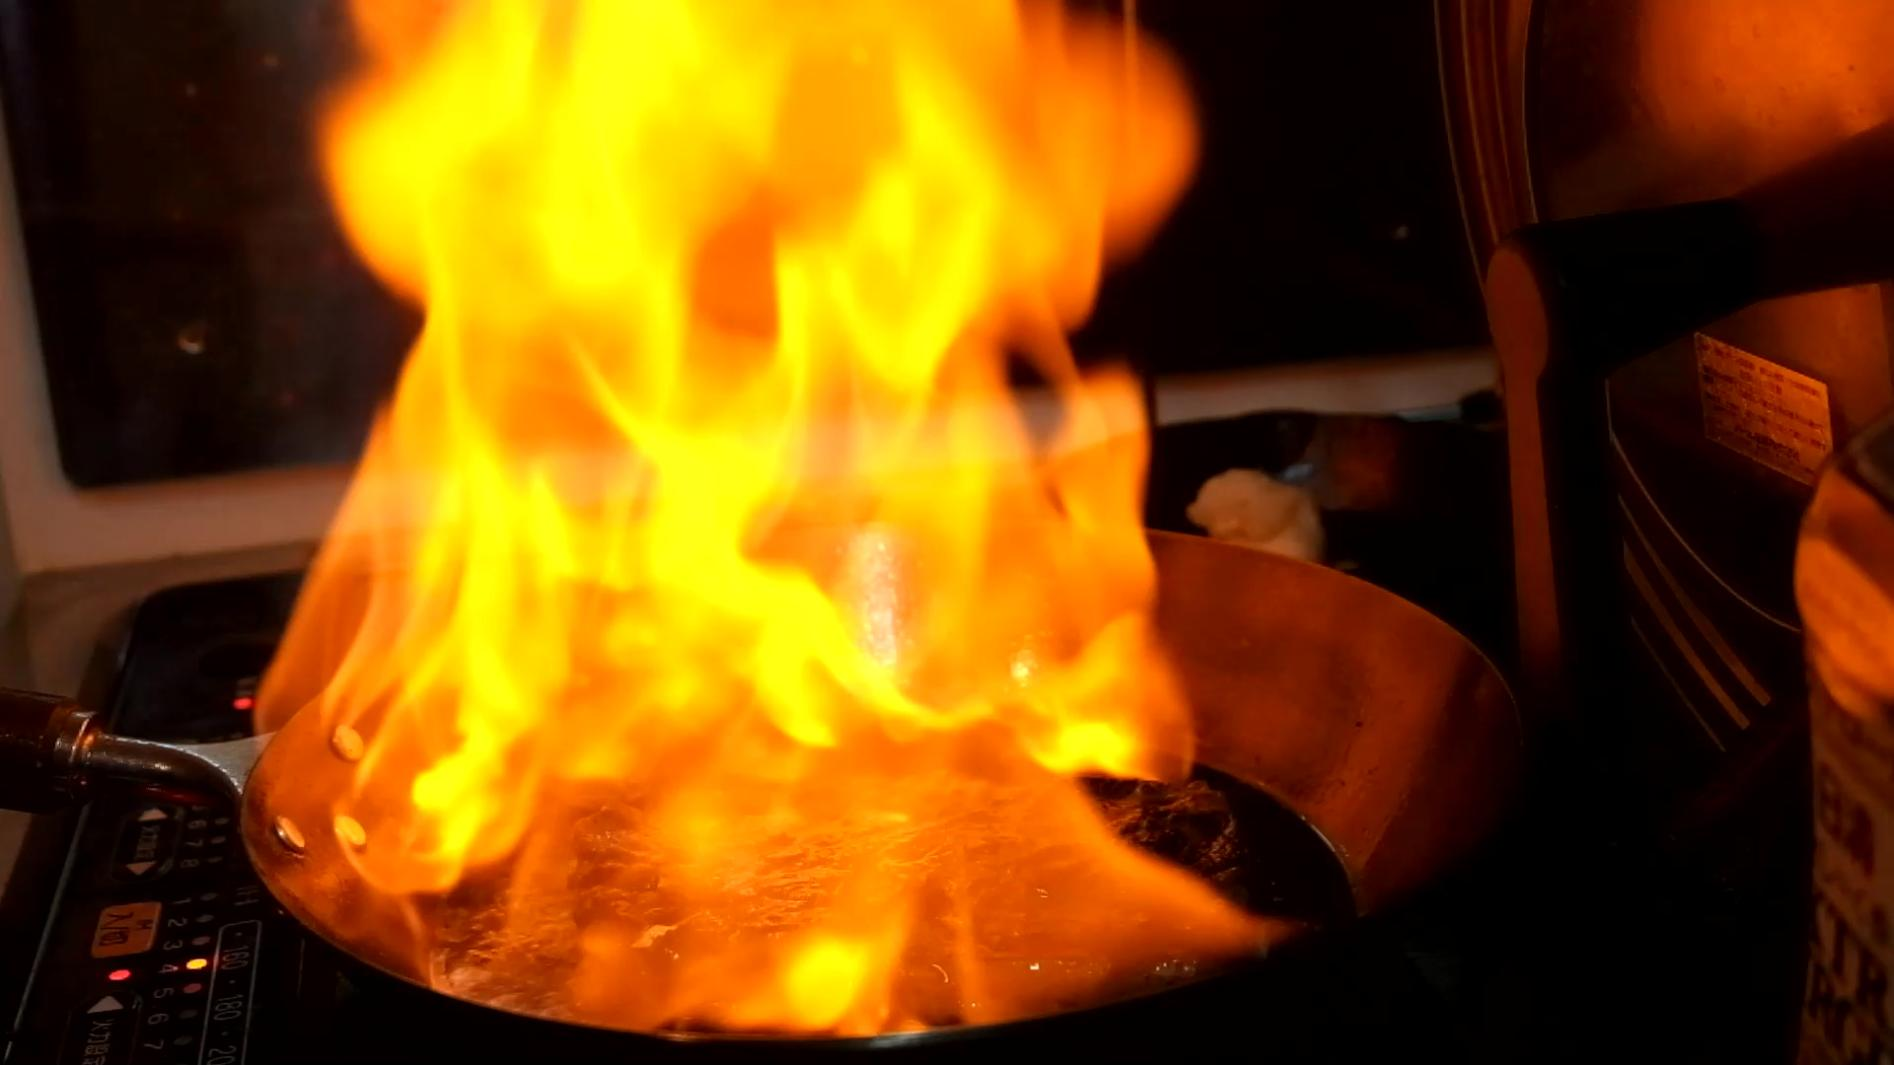
\includegraphics[width=50mm]{pic/pic1.jpg}
                \end{center}
                \caption{下宿先でフランベする図}
                % \label{fig:pic1}
            \end{figure}
        \end{column}
        \begin{column}{0.48\textwidth}
            \begin{figure}[htbp]
                \begin{center}
                    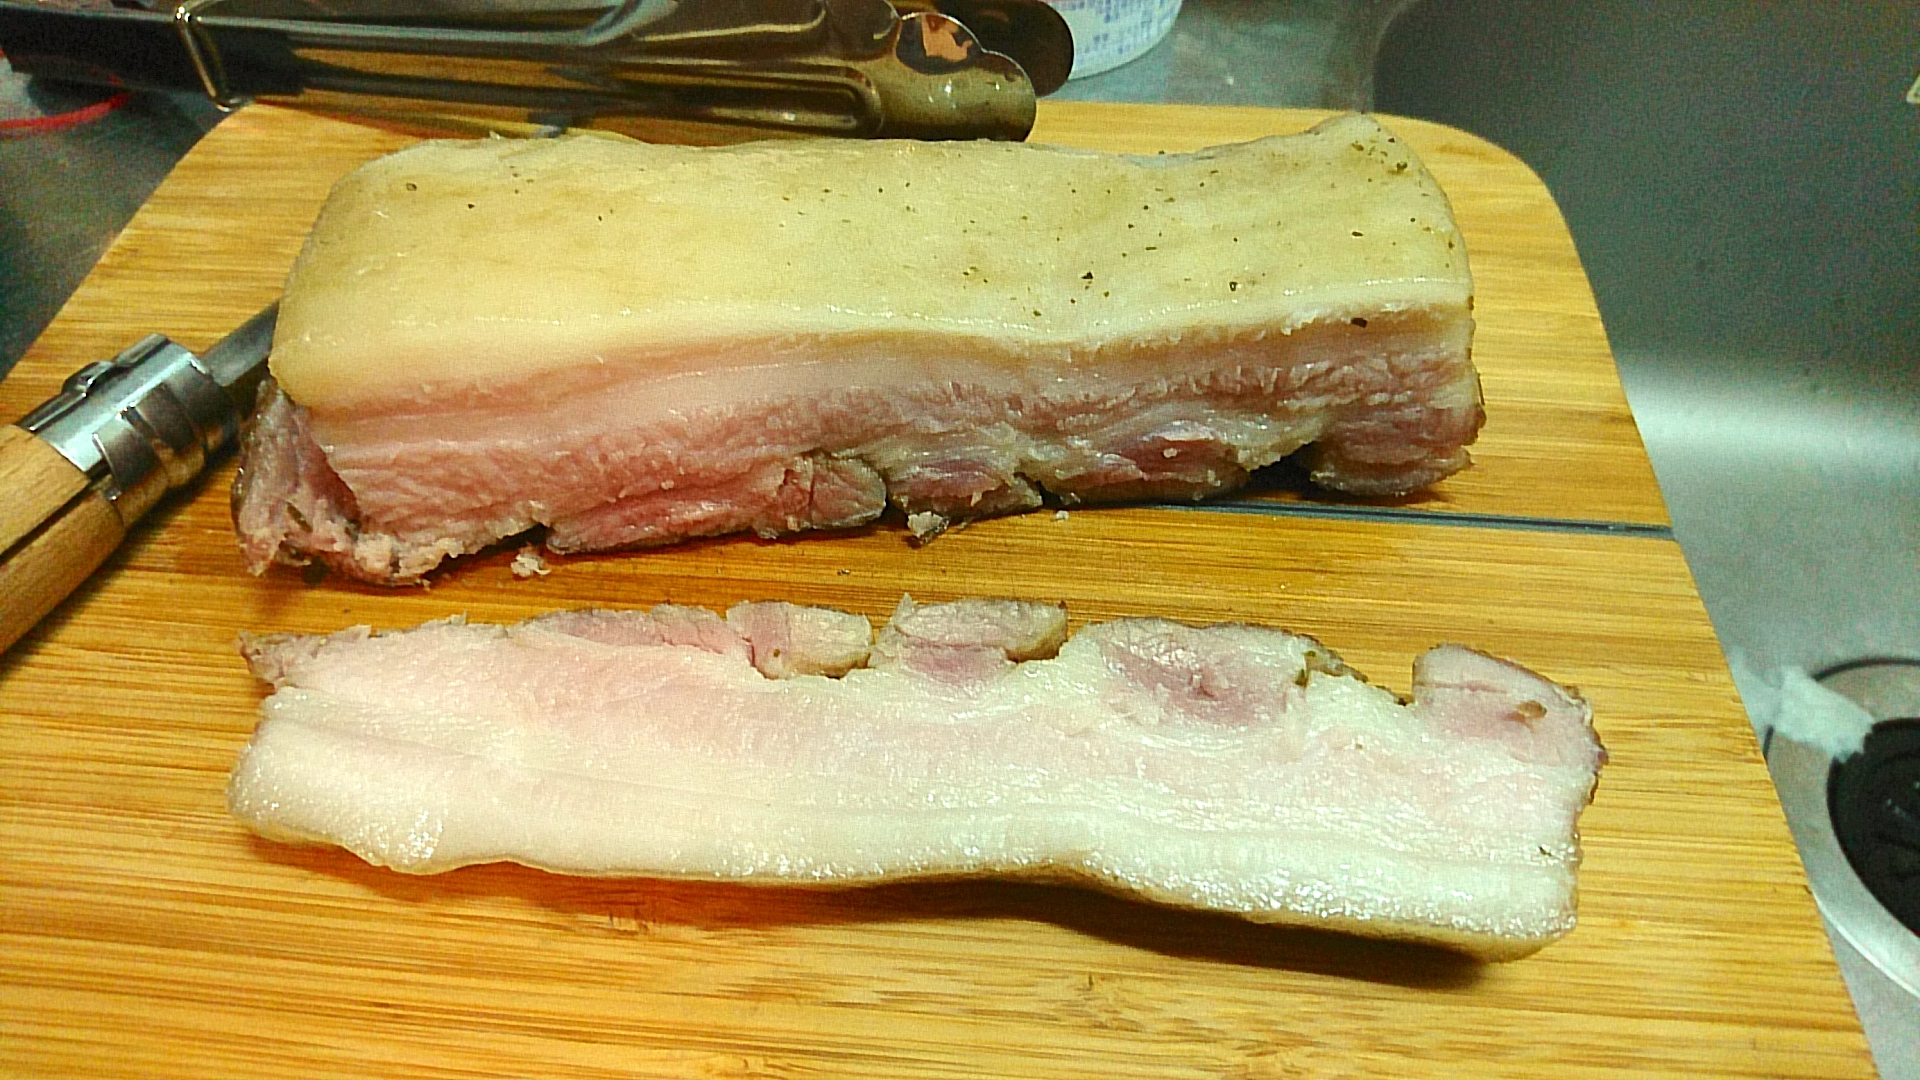
\includegraphics[width=50mm]{pic/pic2.jpg}
                \end{center}
                \caption{自家製ベーコン}
                % \label{fig:pic2}
            \end{figure}
        \end{column}
    \end{columns}
\end{frame}

%%%%%%%%%%%%%%%%%%%%%%%%%%%%%%%%%%%%%%
% 趣味:サイクリング
%%%%%%%%%%%%%%%%%%%%%%%%%%%%%%%%%%%%%%
\begin{frame}
    \frametitle{サイクリング}
    \begin{itemize}
        \item コロナ禍でドライブに行けなかったため,一人で誰にも迷惑をかけず遠くに行きたいと思い,卒論発表後にロードバイクを購入したことがきっかけで始めた.
        \item 今まで行った中で一番遠いところは,岐阜県恵那市(片道約60km)
        \item 1日での最高走行距離は約70km(常滑市まで往復)
    \end{itemize}
    \begin{block}{今後の目標}
        \begin{itemize}
            \item 実家(片道約60km)まで自転車で帰省する.
            \item 琵琶湖をキャンプしながら自転車で一周する
        \end{itemize}
    \end{block}
\end{frame}

%%%%%%%%%%%%%%%%%%%%%%%%%%%%%%%%%%%%%%
% 趣味:キャンプ
%%%%%%%%%%%%%%%%%%%%%%%%%%%%%%%%%%%%%%
\begin{frame}
    \frametitle{キャンプ}
    \begin{itemize}
        \item youtubeで見たブッシュクラフトの動画とアニメ"ゆるキャン△"がきっかけで始めた.
        \item 2018年のアマチュア無線コンテストの時に初めてキャンプをした.
        \item 最近までキャンプ道具を集めるだけになっていた.
        \item ロードバイクを買ったので,キャンプツーリングに行けるようになった.
    \end{itemize}
    \begin{columns}
        \begin{column}{0.48\textwidth}
            \begin{figure}[htbp]
                \begin{center}
                    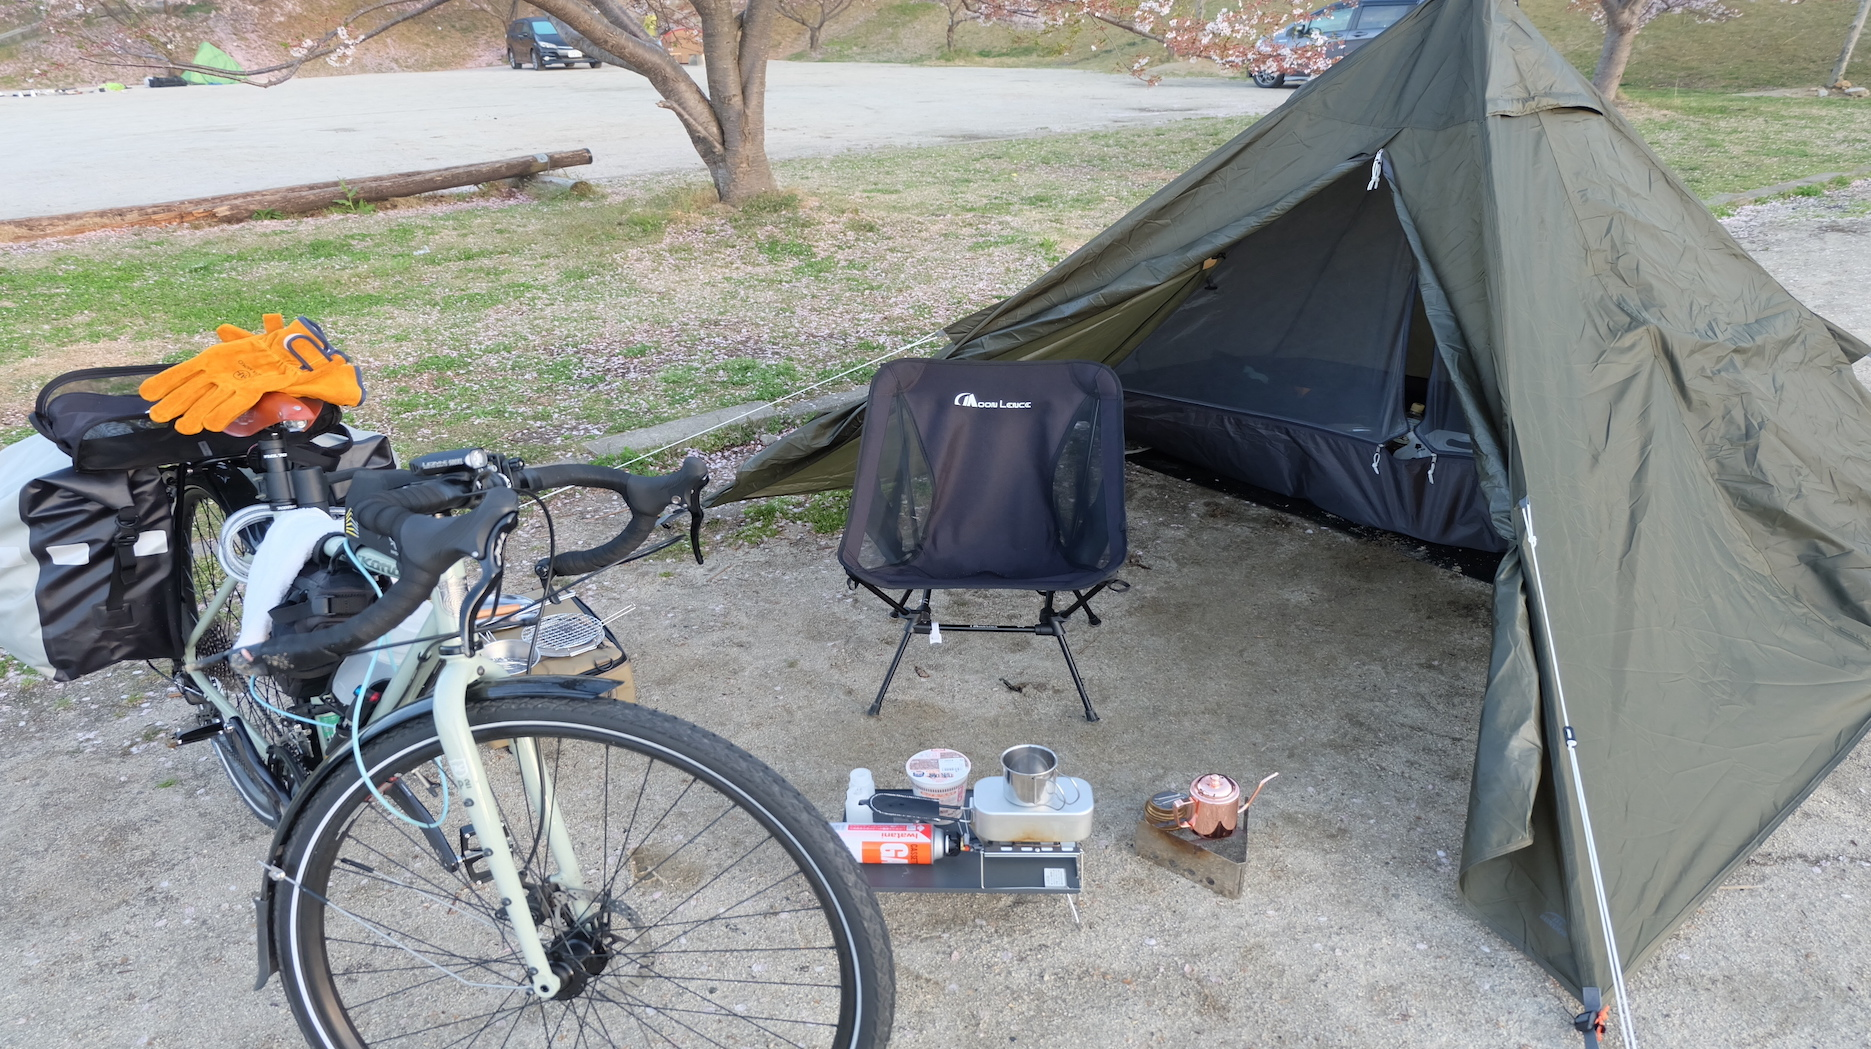
\includegraphics[width=50mm]{pic/pic3.JPG}
                \end{center}
                % \caption{下宿先でフランベする図}
                % \label{fig:pic1}
            \end{figure}
        \end{column}
        \begin{column}{0.48\textwidth}
            \begin{figure}[htbp]
                \begin{center}
                    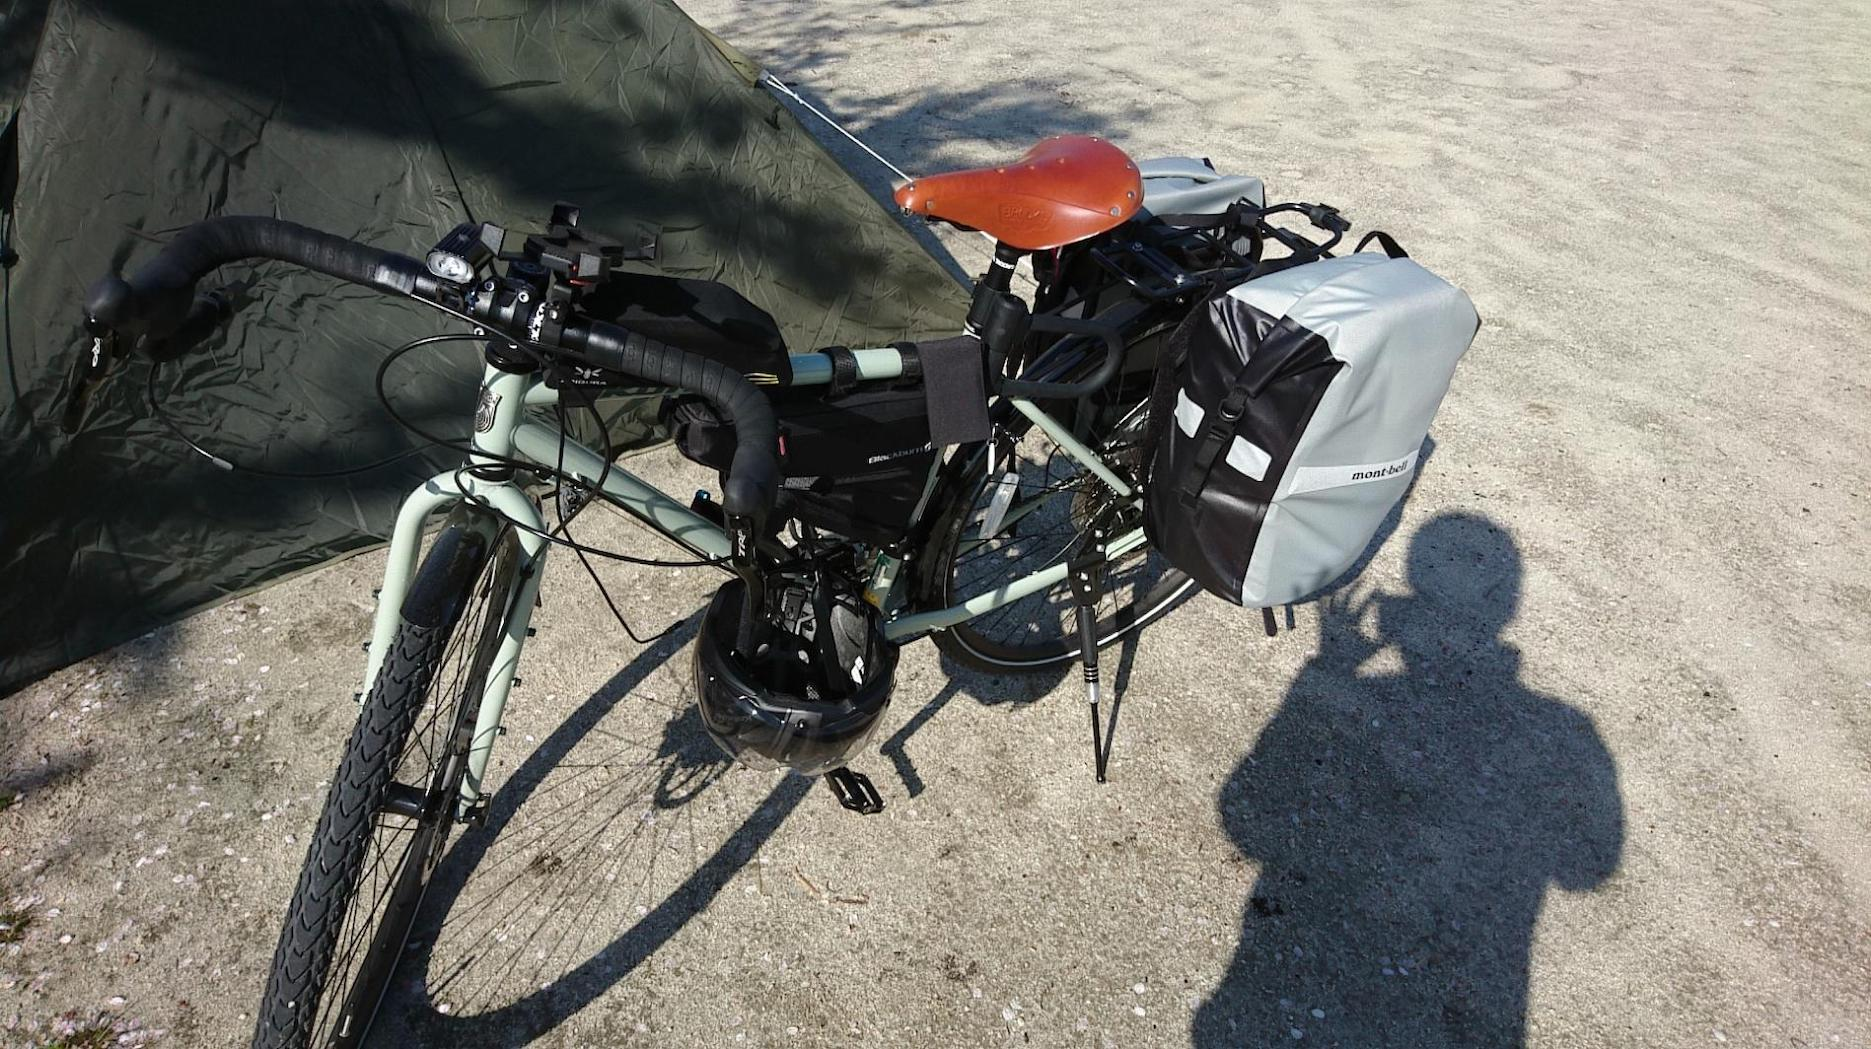
\includegraphics[width=50mm]{pic/pic4.JPG}
                \end{center}
                % \caption{自家製ベーコン}
                % \label{fig:pic2}
            \end{figure}
        \end{column}
    \end{columns}
\end{frame}

%%%%%%%%%%%%%%%%%%%%%%%%%%%%%%%%%%%%%%
% 所属サークル
%%%%%%%%%%%%%%%%%%%%%%%%%%%%%%%%%%%%%%
\begin{frame}
    \frametitle{アマチュア無線研究会}
    \begin{block}{アマチュア無線とは}
        "金銭上の利益のためでなく,もつぱら個人的な無線技術の興味によつて行う自己訓練,通信及び技術的研究の業務をいう."\\
        (電波法施行規則第三条十五)
    \end{block}
    \begin{itemize}
        \item アマチュア無線のコンテストでは,制限時間内での交信数を競う.
        % \item 電波を遠くまで届けるために高いところ(山)に登りに行くことが多い.
        \item 無線以外に電子工作やプログラミング,サーバー管理といったこともしている.
    \end{itemize}
    \begin{columns}
        \begin{column}{0.48\textwidth}
            \begin{figure}[htbp]
                \begin{center}
                    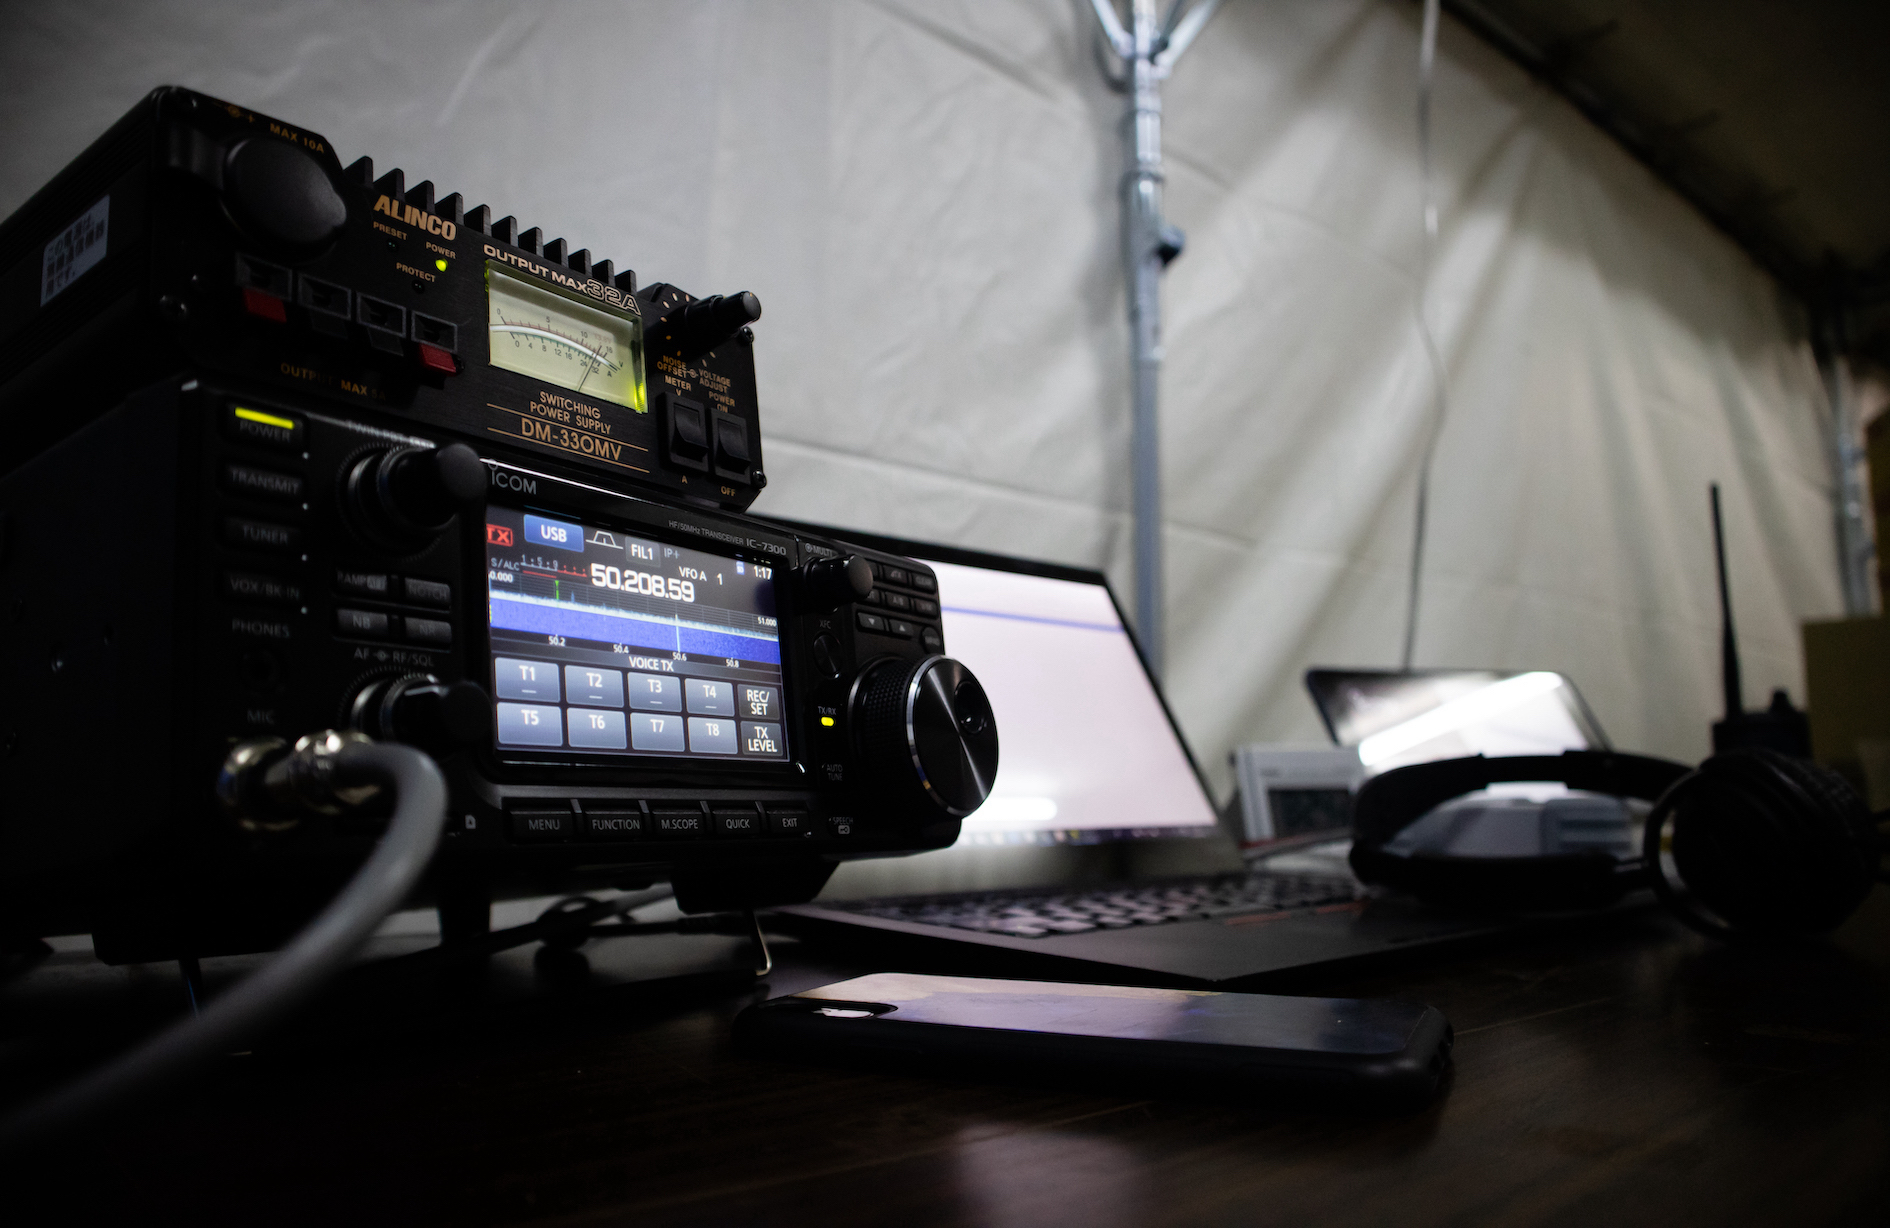
\includegraphics[width=.9\hsize]{pic/pic5.JPG}
                \end{center}
                % \caption{下宿先でフランベする図}
                % \label{fig:pic1}
            \end{figure}
        \end{column}
        \begin{column}{0.48\textwidth}
            \begin{figure}[htbp]
                \begin{center}
                    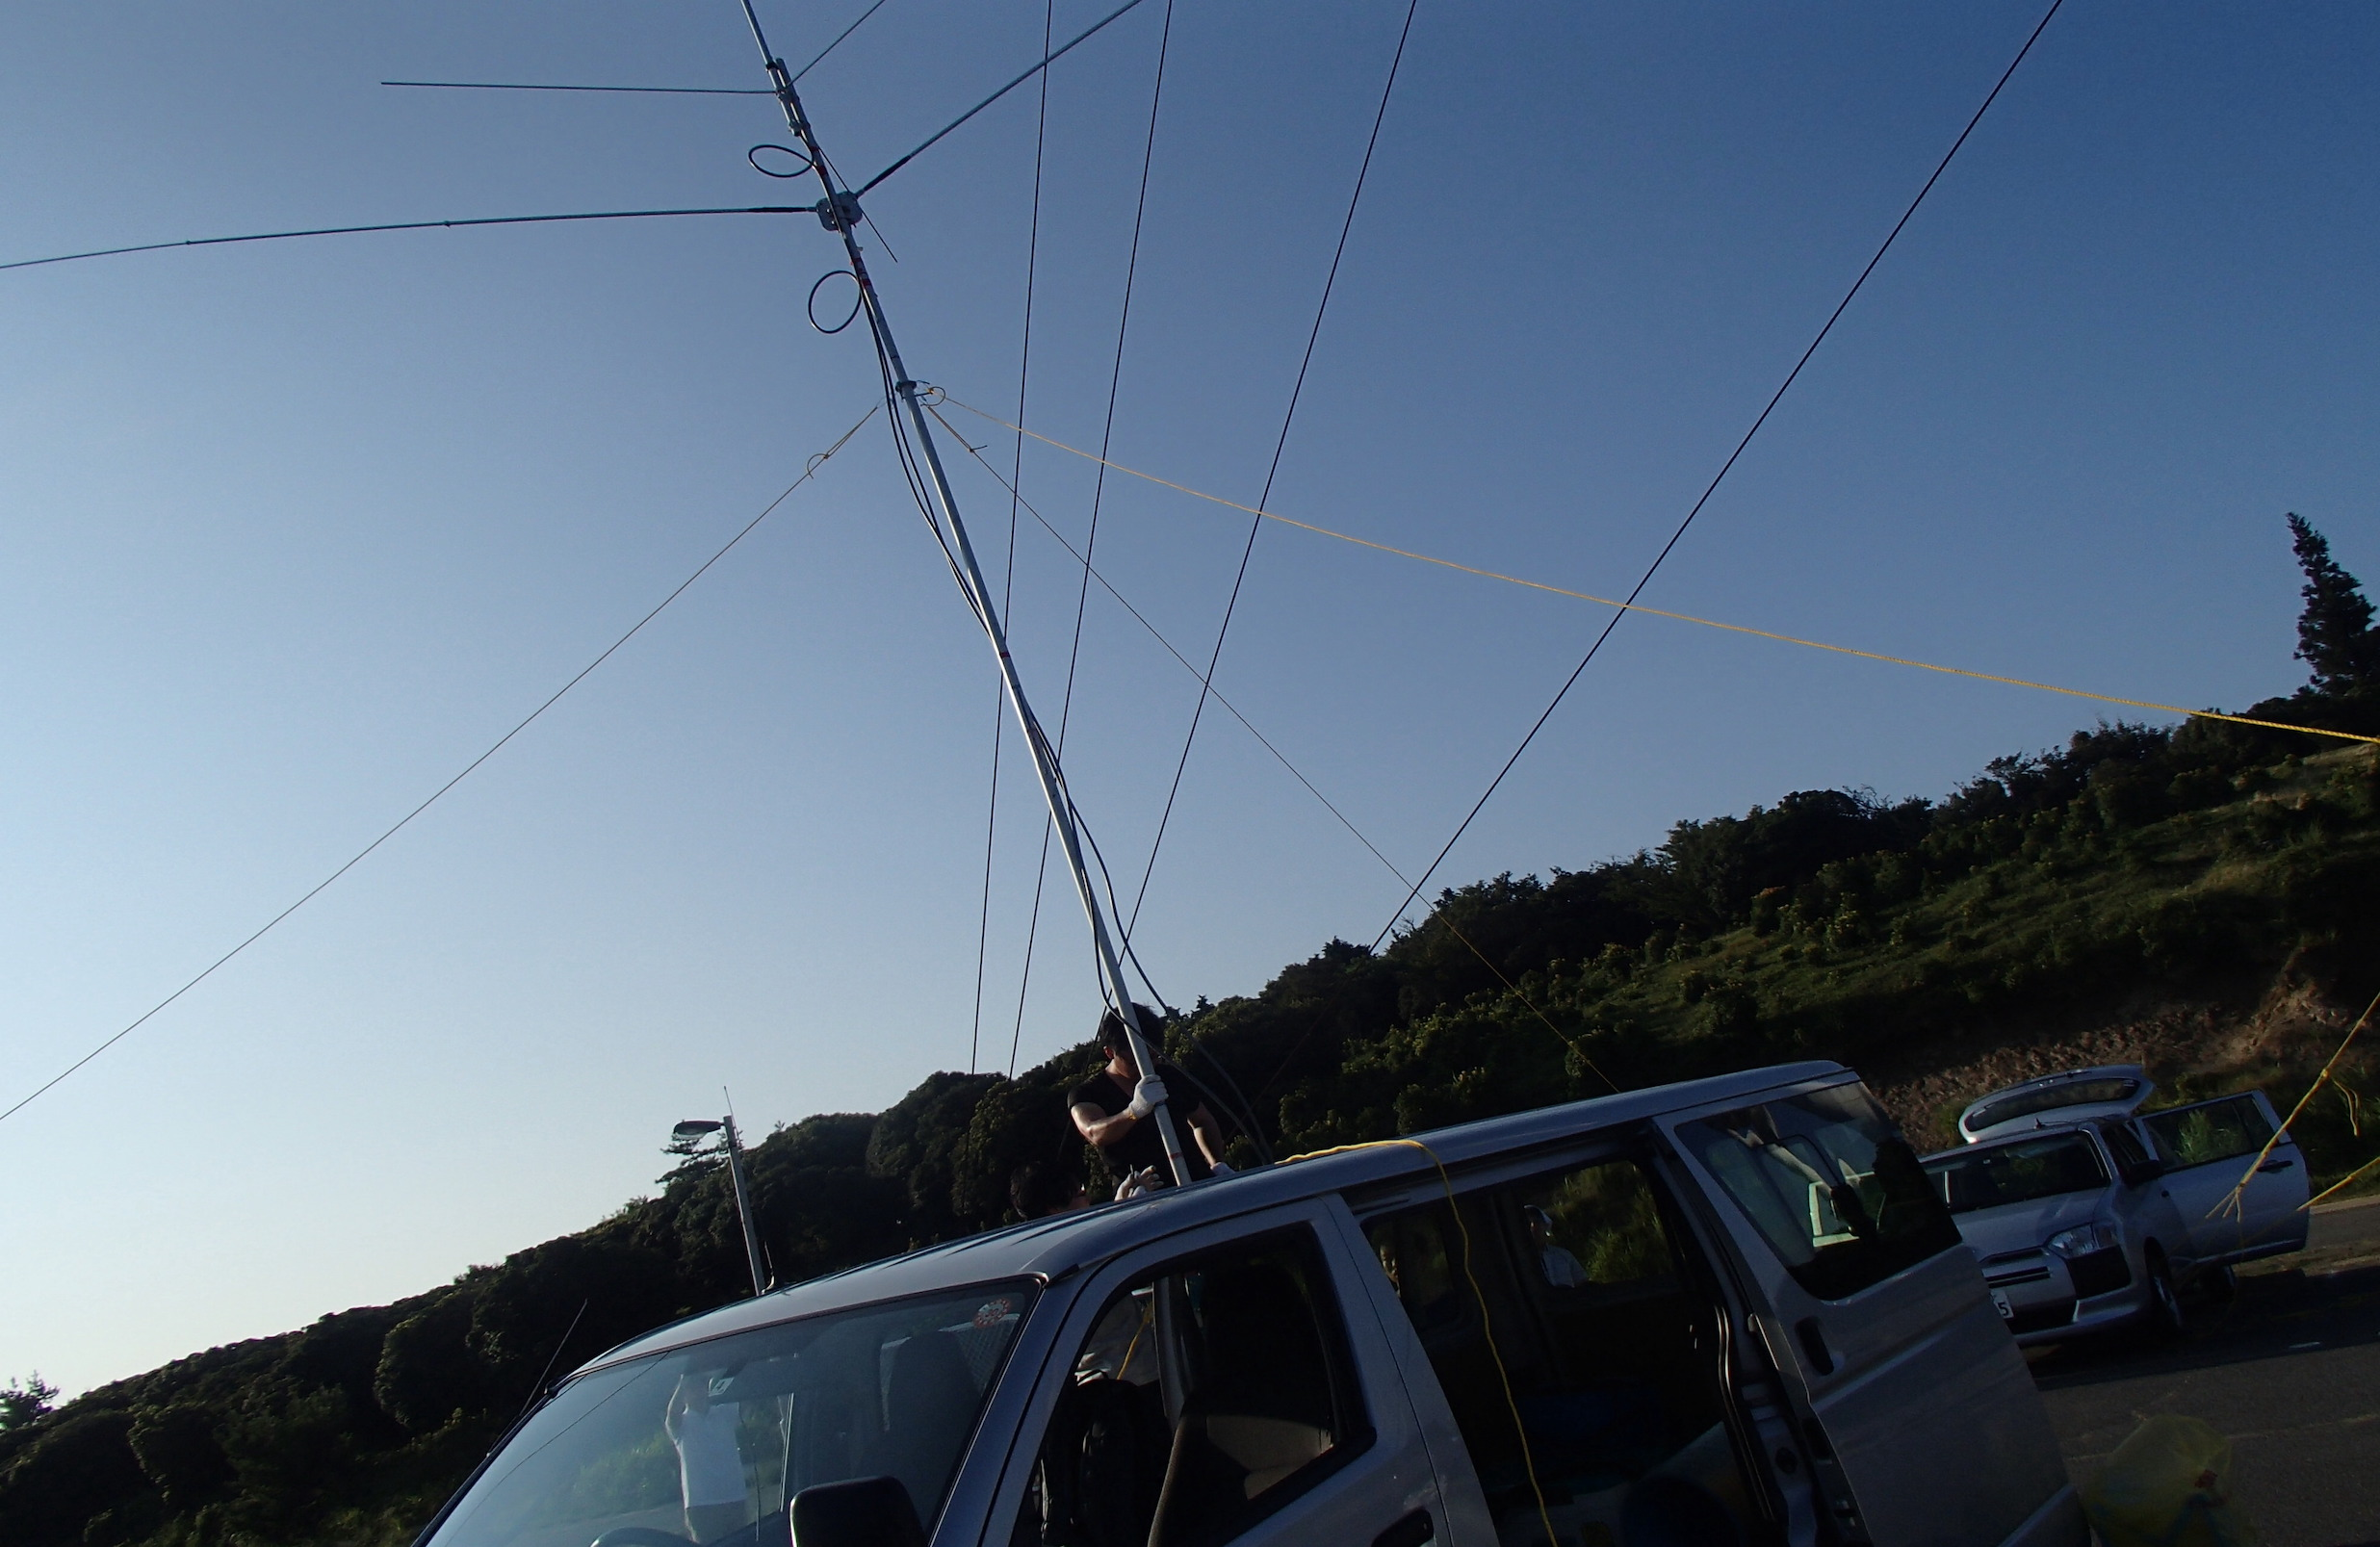
\includegraphics[width=.9\hsize]{pic/pic6.JPG}
                \end{center}
                % \caption{自家製ベーコン}
                % \label{fig:pic2}
            \end{figure}
        \end{column}
    \end{columns}
\end{frame}

%%% Local Variables:
%%% mode: japanese-latex
%%% TeX-master: "kosuge_slide"
%%% End:


%%%%%%%%%%%%%%%%%%%%%%%%%%%%%%%%%%%%%%
% 背景理論付きSAT
%%%%%%%%%%%%%%%%%%%%%%%%%%%%%%%%%%%%%%
\begin{frame}
  \frametitle{背景理論付きSAT {\large (Satisfiability Modulo Theories; SMT)}}
  \begin{alertblock}{}
    \alert{\bf SMT} は等号や算術,配列やリスト,ビットベクターなど様々な背景理論が
    扱えるように,SAT を拡張・発展させた技術である.
  \end{alertblock}
  \bigskip
  \begin{itemize}
  \item SMT の特長は,背景理論を表現能力の高い述語論理で記述できるため,
    問題を簡潔に記述できる点である.
  \item 近年,Z3ソルバー (Microsoft Research) などの高速 SMT ソルバー
    が開発され,プログラム検証,定理証明,制約充足問題など,様々な分野
    への応用が急速に拡大している.
  \item 一方で,\alert{\bf 制約充足問題}に対する SMT ソルバーの求解性
    能は,SAT 型制約ソルバーと比べて劣るとの報告[Soh+2017]もあり,
    改良の余地が残っている.
  \end{itemize}
\end{frame}
%%%%%%%%%%%%%%%%%%%%%%%%%%%%%%%%%%%%%%
% \distinct 制約
%%%%%%%%%%%%%%%%%%%%%%%%%%%%%%%%%%%%%%
\begin{frame}
  \frametitle{{\distinct}制約と制約充足問題}
  \begin{alertblock}{}
    \bm{$$distinct(x_{1},x_{2},\ldots, x_{n})$$}
    {\distinct}制約は,整数上の変数$x_{i}$が互いに異なることを表す制約
    である.
  \end{alertblock}
  \begin{itemize}
  \item この制約は,
    $$\bigwedge_{1 \leq i < j \leq n} x_i \neq x_j$$
    を意味する.
  \item {\distinct}制約は,時間割問題,グラフ彩色問題,組合せデザイン
    など様々な制約充足問題に現れる.
  \item そのような問題に対し,{\distinct}制約を効率良く解くことは重要
    な研究課題である.
  \end{itemize}
\end{frame}
%%%%%%%%%%%%%%%%%%%%%%%%%%%%%%%%%%%%%%
% クイーングラフ彩色問題
%%%%%%%%%%%%%%%%%%%%%%%%%%%%%%%%%%%%%%
\begin{frame}
  \frametitle{{\distinct}制約が現れる制約充足問題の例}
  \begin{block}{クイーングラフ彩色問題}
    $N$個ずつの$N$個のグループからなるクイーン (計$N^2$個) を,
    $N\times N$のチェス盤に,同じグループのクイーン同士が互いに取られ
    ないように配置する問題
  \end{block}
  \begin{center}
\scalebox{0.8}{
    \begin{tikzpicture}
        \fill[red]    (0.5,0.5) circle (0.25);
        \fill[red]    (1.5,2.5) circle (0.25);
        \fill[red]    (2.5,4.5) circle (0.25);
        \fill[red]    (3.5,1.5) circle (0.25);
        \fill[red]    (4.5,3.5) circle (0.25);
        \fill[blue]   (0.5,3.5) circle (0.25);
        \fill[blue]   (1.5,0.5) circle (0.25);
        \fill[blue]   (2.5,2.5) circle (0.25);
        \fill[blue]   (3.5,4.5) circle (0.25);
        \fill[blue]   (4.5,1.5) circle (0.25);
        \fill[green]  (0.5,1.5) circle (0.25);
        \fill[green]  (1.5,3.5) circle (0.25);
        \fill[green]  (2.5,0.5) circle (0.25);
        \fill[green]  (3.5,2.5) circle (0.25);
        \fill[green]  (4.5,4.5) circle (0.25);
        \fill[black] (0.5,4.5) circle (0.25);
        \fill[black] (1.5,1.5) circle (0.25);
        \fill[black] (2.5,3.5) circle (0.25);
        \fill[black] (3.5,0.5) circle (0.25);
        \fill[black] (4.5,2.5) circle (0.25);
        \fill[pink] (0.5,2.5) circle (0.25);
        \fill[pink] (1.5,4.5) circle (0.25);
        \fill[pink] (2.5,1.5) circle (0.25);
        \fill[pink] (3.5,3.5) circle (0.25);
        \fill[pink] (4.5,0.5) circle (0.25);
        \draw [step=10mm] (0,0) grid (5,5);
        \node at (2.5, 0) [below] {N=5のとき};
    \end{tikzpicture}
}
\end{center}

  \begin{itemize}
  \item この問題は{\distinct}制約のみを用いて記述できる.
  \item Knuthの教科書 The Art of Computer Programming でも
    取り上げられている.
  \end{itemize}
\end{frame}
%%%%%%%%%%%%%%%%%%%%%%%%%%%%%%%%%%%%%%
% 研究概要
%%%%%%%%%%%%%%%%%%%%%%%%%%%%%%%%%%%%%%
\begin{frame}\frametitle{研究概要}
  \begin{alertblock}{研究目的}
    クイーングラフ彩色問題を題材とし,
    SATの手法を参考に,
    SMT の{\distinct}制約を
    高速化するための様々な方法を実装し,比較評価する.
  \end{alertblock}
   %
  \begin{block}{研究内容}
    \begin{enumerate}
    \item \structure{クイーングラフ彩色問題に対し,4種類のSMT符号化を実装}
      \begin{itemize}
      \item \alert{\bf 色変数モデル (COL)}
      \item \alert{\bf 位置変数モデル (POS)}
      \item 0-1変数モデル (PB)
      \item ハイブリッドモデル (COL+PB, POS+PB)
      \end{itemize}
    \item \structure{SATの手法を参考に,\bm{\distinct}制約の高速化手法をSMTで実装}
      \begin{itemize}
      \item \alert{\bf 鳩の巣原理を用いたヒント制約 (H1)}
      \item at-least-one 制約を用いたヒント制約 (H2)
      \item {\distinct}制約の擬似ブール符号化 (O1, O2)
      \end{itemize}
    \item \structure{クイーングラフ彩色問題($5\leq N\leq 13$)を用いた評価実験}
    \end{enumerate}
  \end{block}
\end{frame}
%%%%%%%%%%%%%%%%%%%%%%%%%%%%%%%%%%%%%%
% 色変数モデルと位置変数モデル
%%%%%%%%%%%%%%%%%%%%%%%%%%%%%%%%%%%%%%
\begin{frame}
  \frametitle{色変数モデル(COL)と位置変数モデル(POS)}

  \begin{itemize}
  \item \structure{色変数モデル(COL)}は,クイーンの色を整数変数とした
    定式化
  \item \structure{位置変数モデル(POS)}は,各行に配置されているクイー
    ンの列番号を整数変数とした定式化
  \end{itemize}
  \begin{center}
    \scalebox{0.7}{\begin{center}
\scalebox{0.4}{
    \begin{tikzpicture}
        \fill[red]    (0.5,0.5) circle (0.25);
        \fill[red]    (1.5,2.5) circle (0.25);
        \fill[red]    (2.5,4.5) circle (0.25);
        \fill[red]    (3.5,1.5) circle (0.25);
        \fill[red]    (4.5,3.5) circle (0.25);
        \fill[blue]   (0.5,3.5) circle (0.25);
        \fill[blue]   (1.5,0.5) circle (0.25);
        \fill[blue]   (2.5,2.5) circle (0.25);
        \fill[blue]   (3.5,4.5) circle (0.25);
        \fill[blue]   (4.5,1.5) circle (0.25);
        \fill[green]  (0.5,1.5) circle (0.25);
        \fill[green]  (1.5,3.5) circle (0.25);
        \fill[green]  (2.5,0.5) circle (0.25);
        \fill[green]  (3.5,2.5) circle (0.25);
        \fill[green]  (4.5,4.5) circle (0.25);
        \fill[black] (0.5,4.5) circle (0.25);
        \fill[black] (1.5,1.5) circle (0.25);
        \fill[black] (2.5,3.5) circle (0.25);
        \fill[black] (3.5,0.5) circle (0.25);
        \fill[black] (4.5,2.5) circle (0.25);
        \fill[pink] (0.5,2.5) circle (0.25);
        \fill[pink] (1.5,4.5) circle (0.25);
        \fill[pink] (2.5,1.5) circle (0.25);
        \fill[pink] (3.5,3.5) circle (0.25);
        \fill[pink] (4.5,0.5) circle (0.25);
        \draw [step=10mm] (0,0) grid (5,5);
        \node at (2.5, 0) [below] {N=5のとき(COL)};
        \node at ( 0,4.5) [left] {0};
        \node at ( 0,3.5) [left] {1};
        \node at ( 0,2.5) [left] {2};
        \node at ( 0,1.5) [left] {3};
        \node at ( 0,0.5) [left] {4};
        \node at (4.5, 5) [above] {4};
        \node at (3.5, 5) [above] {3};
        \node at (2.5, 5) [above] {2};
        \node at (1.5, 5) [above] {1};
        \node at (0.5, 5) [above] {0};
        %
        %
        %
        %
        \foreach \y / \x in {4.5/7.5, 2.5/8.5, 0.5/9.5, 3.5/10.5, 1.5/11.5}
        {
        \node at (\x,\y) {0};
        }
        \foreach \y / \x in {1.5/7.5, 4.5/8.5, 2.5/9.5, 0.5/10.5, 3.5/11.5}
        {
        \node at (\x,\y) {1};
        }
        \foreach \y / \x in {3.5/7.5, 1.5/8.5, 4.5/9.5, 2.5/10.5, 0.5/11.5}
        {
        \node at (\x,\y) {2};
        }
        \foreach \y / \x in {0.5/7.5, 3.5/8.5, 1.5/9.5, 4.5/10.5, 2.5/11.5}
        {
        \node at (\x,\y) {3};
        }
        \foreach \y / \x in {2.5/7.5, 0.5/8.5, 3.5/9.5, 1.5/10.5, 4.5/11.5}
        {
        \node at (\x,\y) {4};
        }
        \draw [step=10mm] (7,0) grid (12,5);
        \node at (9.5, 0) [below] {N=5のとき(POS)};
        \node at ( 7,4.5) [left] {0};
        \node at ( 7,3.5) [left] {1};
        \node at ( 7,2.5) [left] {2};
        \node at ( 7,1.5) [left] {3};
        \node at ( 7,0.5) [left] {4};
        \fill[black] ( 7.5,5.5) circle (0.25);
        \fill[pink]  ( 8.5,5.5) circle (0.25);
        \fill[red]   ( 9.5,5.5) circle (0.25);
        \fill[blue]  (10.5,5.5) circle (0.25);
        \fill[green] (11.5,5.5) circle (0.25);
    \end{tikzpicture}
}
\end{center}
}
  \end{center}
\end{frame}
%%%%%%%%%%%%%%%%%%%%%%%%%%%%%%%%%%%%%% 
% 位置変数モデル
%%%%%%%%%%%%%%%%%%%%%%%%%%%%%%%%%%%%%%
\begin{frame}\frametitle{位置変数モデル(POS)}
  $N$次クイーングラフ彩色問題に対して,集合$\bm{N}$を
  次のように定義する.
\begin{eqnarray*}
  \bm{N} &=& \{0,1,\ldots,N-1\}
\end{eqnarray*}
\vskip -0.5em
\begin{itemize}
\item $\bm{N}$は,行番号$i$, 列番号$j$, クイーンの色$k$の取り得る値の集合
% \item $\bm{U}$は,$i+j$の取り得る値の集合,右上がりの対角線に対応
% \item $\bm{D}$は,$i-j$の取り得る値の集合,右下がりの対角線に対応
\end{itemize}
\begin{exampleblock}{$N$次クイーングラフ彩色問題の定式化}
  \[
    \begin{array}{lr}
      y_{ik}\in\bm{N} & (i,k\in\bm{N})\\
      distinct~\{y_{ik} \mid k\in\bm{N}\} & (i\in\bm{N})\\
      distinct~\{y_{ik} \mid i\in\bm{N}\} & (k\in\bm{N})\\
      distinct~\{y_{ik} + i\mid i\in\bm{N}\} & (k\in\bm{N})\\
      distinct~\{y_{ik} - i\mid i\in\bm{N}\} & (k\in\bm{N})
    \end{array}
  \]  
\end{exampleblock}
\begin{itemize}
\item 整数変数$y_{ik}$ の値は,色$k$のクイーンが行$i$で配置されている
  列番号を表す.
\end{itemize}
\end{frame}
%%%%%%%%%%%%%%%%%%%%%%%%%%%%%%%%%%%%%% 
% 位置変数モデル
%%%%%%%%%%%%%%%%%%%%%%%%%%%%%%%%%%%%%%
% \begin{frame}
%   \frametitle{位置変数モデル}
% %  \begin{center}
\scalebox{0.4}{
    \begin{tikzpicture}
        \fill[red]    (0.5,0.5) circle (0.25);
        \fill[red]    (1.5,2.5) circle (0.25);
        \fill[red]    (2.5,4.5) circle (0.25);
        \fill[red]    (3.5,1.5) circle (0.25);
        \fill[red]    (4.5,3.5) circle (0.25);
        \fill[blue]   (0.5,3.5) circle (0.25);
        \fill[blue]   (1.5,0.5) circle (0.25);
        \fill[blue]   (2.5,2.5) circle (0.25);
        \fill[blue]   (3.5,4.5) circle (0.25);
        \fill[blue]   (4.5,1.5) circle (0.25);
        \fill[green]  (0.5,1.5) circle (0.25);
        \fill[green]  (1.5,3.5) circle (0.25);
        \fill[green]  (2.5,0.5) circle (0.25);
        \fill[green]  (3.5,2.5) circle (0.25);
        \fill[green]  (4.5,4.5) circle (0.25);
        \fill[black] (0.5,4.5) circle (0.25);
        \fill[black] (1.5,1.5) circle (0.25);
        \fill[black] (2.5,3.5) circle (0.25);
        \fill[black] (3.5,0.5) circle (0.25);
        \fill[black] (4.5,2.5) circle (0.25);
        \fill[pink] (0.5,2.5) circle (0.25);
        \fill[pink] (1.5,4.5) circle (0.25);
        \fill[pink] (2.5,1.5) circle (0.25);
        \fill[pink] (3.5,3.5) circle (0.25);
        \fill[pink] (4.5,0.5) circle (0.25);
        \draw [step=10mm] (0,0) grid (5,5);
        \node at (2.5, 0) [below] {N=5のとき(COL)};
        \node at ( 0,4.5) [left] {0};
        \node at ( 0,3.5) [left] {1};
        \node at ( 0,2.5) [left] {2};
        \node at ( 0,1.5) [left] {3};
        \node at ( 0,0.5) [left] {4};
        \node at (4.5, 5) [above] {4};
        \node at (3.5, 5) [above] {3};
        \node at (2.5, 5) [above] {2};
        \node at (1.5, 5) [above] {1};
        \node at (0.5, 5) [above] {0};
        %
        %
        %
        %
        \foreach \y / \x in {4.5/7.5, 2.5/8.5, 0.5/9.5, 3.5/10.5, 1.5/11.5}
        {
        \node at (\x,\y) {0};
        }
        \foreach \y / \x in {1.5/7.5, 4.5/8.5, 2.5/9.5, 0.5/10.5, 3.5/11.5}
        {
        \node at (\x,\y) {1};
        }
        \foreach \y / \x in {3.5/7.5, 1.5/8.5, 4.5/9.5, 2.5/10.5, 0.5/11.5}
        {
        \node at (\x,\y) {2};
        }
        \foreach \y / \x in {0.5/7.5, 3.5/8.5, 1.5/9.5, 4.5/10.5, 2.5/11.5}
        {
        \node at (\x,\y) {3};
        }
        \foreach \y / \x in {2.5/7.5, 0.5/8.5, 3.5/9.5, 1.5/10.5, 4.5/11.5}
        {
        \node at (\x,\y) {4};
        }
        \draw [step=10mm] (7,0) grid (12,5);
        \node at (9.5, 0) [below] {N=5のとき(POS)};
        \node at ( 7,4.5) [left] {0};
        \node at ( 7,3.5) [left] {1};
        \node at ( 7,2.5) [left] {2};
        \node at ( 7,1.5) [left] {3};
        \node at ( 7,0.5) [left] {4};
        \fill[black] ( 7.5,5.5) circle (0.25);
        \fill[pink]  ( 8.5,5.5) circle (0.25);
        \fill[red]   ( 9.5,5.5) circle (0.25);
        \fill[blue]  (10.5,5.5) circle (0.25);
        \fill[green] (11.5,5.5) circle (0.25);
    \end{tikzpicture}
}
\end{center}

%   {\small
%     各行に配置される\alert{クイーンの列番号}を整数変数とした制約モデル
%   }
%   {\footnotesize
%     \setlength{\abovedisplayskip}{1pt} % 上部のマージン
%     \setlength{\belowdisplayskip}{0pt} % 下部のマージン
%     \begin{block}{}
%       \setlength{\itemsep}{0pt}
%       \setlength{\parskip}{0pt}
%       \begin{itemize}
%       \item 色$k$のクイーンが行$i$で配置されている列番号を整数変数$y_{ik} \in \bf N (i, k \in \bf N)$で表す
%       \item 同一の\alert{行番号}に同色のクイーンが配置されないことより
%         $$distinct\{y_{ik} | k \in \bf N\} \; (i \in \bf N)$$
%       \item 同一の\alert{列番号}に同色のクイーンが配置されないことより
%         $$distinct\{y_{ik} | i \in \bf N\} \; (k \in \bf N)$$
%       \item \alert{右上がりの対角線上}に2つ以上の同色のクイーンが配置されないことより
%         $$distinct\{y_{ik}+i | i \in \bf N\} \; (k \in \bf N)$$
%       \item \alert{右下がりの対角線上}に2つ以上の同色のクイーンが配置されないことより
%         $$distinct\{y_{ik}-i | i \in \bf N\} \; (k \in \bf N)$$
%       \end{itemize}
%     \end{block}
%   }
% \end{frame}
%%%%%%%%%%%%%%%%%%%%%%%%%%%%%%%%%%%%%%
% 高速化手法1
%%%%%%%%%%%%%%%%%%%%%%%%%%%%%%%%%%%%%%
\begin{frame}
  \frametitle{鳩の巣原理を用いたヒント制約(H1)~[田島・田村,2008]}
  SAT符号化された{\distinct}制約に,鳩の巣原理を用いたヒントを加える
  と求解速度が向上することが知られている.
  \begin{block}{}
    $distinct(x_{1},\ldots,x_{n})$について,$x_i \in
    \{\ell,\ell+1,\ldots,u\}$であるとき,以下の2つの制約を追加する.
    \[
      \bigvee_{i=1}^{n}x_{i}\geq \ell+n-1 \qquad
      \bigvee_{i=1}^{n}x_{i}\leq u-n+1
    \]
  \end{block}
  \begin{exampleblock}{例}
    $distinct(x_1, x_2, x_3)$について, $x_i \in \{1,2,3\}$であ
    るとき,以下の制約が追加される.
    \vspace{-3mm}
    \begin{eqnarray*}
      (x_1\geq 3) \lor (x_2 \geq 3) \lor (x_3 \geq 3)\\
      (x_1\leq 1) \lor (x_2 \leq 1) \lor (x_3 \leq 1)
    \end{eqnarray*}
  \end{exampleblock}
\end{frame}
%%%%%%%%%%%%%%%%%%%%%%%%%%%%%%%%%%%%%%
% 実験概要2
%%%%%%%%%%%%%%%%%%%%%%%%%%%%%%%%%%%%%%
\begin{frame}\frametitle{実験概要}
  実装した SMT符号化および{\distinct}制約の高速化手法を評価するために,
  以下の実験を行った.
  \bigskip
  \begin{itemize}
  \item \structure{比較に用いた実装 (3種類,11個)}\footnote{%
    予備実験で性能が悪かったハイブリッドモデル(計6個)は省略}
    \begin{itemize}
    \item 色変数モデル(4個): COL, COL+H1, COL+H2, COL+H1+H2
    \item 0-1変数モデル(3個): PB, PB+O1, PB+O2
    \item 位置変数モデル(4個): POS, POS+H1, POS+H2, POS+H1+H2
    \end{itemize}
  \item \structure{ベンチマーク問題}: $N$次クイーングラフ彩色問題 ($5\leq N\leq 13$)
  \item \structure{SMTソルバー}: Z3 ver.4.8.9
  \item \structure{制限時間}: 1問あたり2時間
  \item \structure{実験環境}: Mac mini, 3.2GHz, 64GB メモリ
  \end{itemize}
\end{frame}
%%%%%%%%%%%%%%%%%%%%%%%%%%%%%%%%%%%%%%
% 実験結果
%%%%%%%%%%%%%%%%%%%%%%%%%%%%%%%%%%%%%%
\begin{frame}
  \frametitle{実験結果: 求解に要したCPU時間 (秒)}
  \begin{block}{}\centering
    {\tiny \begin{tabular}{l|rr|rr} 
  & \multicolumn{2}{c|}{基本ソルバー} & \multicolumn{2}{c}{改良ソルバー} \\
  & \code{changed} & \code{unchanged} & \code{changed} & \code{unchanged} \\ \hline
  解けた問題数(到達可能) & 11 & 11 & 11 & 11 \\
  解けた問題数(到達不能) & 10 & 10 & 56 & \alert{60} \\\hline
  平均 CPU 時間(秒) & 223.796 & 151.341 & 101.758 & \alert{59.095} \\
\end{tabular}}
  \end{block}
  \begin{itemize}
  \item {\distinct}制約に対するヒントがない状態で比較すると,
    位置変数モデル(POS)の性能が良い.
  \item ヒントの有無で比較すると,ヒント有が$N=11$を解けていることか
    ら,ヒントは有効に働いていることがわかる.
  \item ヒントがある状態で見ると,位置変数モデル(POS)が,色変数モデル
    (COL)より,CPU時間が短い.
  \end{itemize}
\end{frame}
%%%%%%%%%%%%%%%%%%%%%%%%%%%%%%%%%%%%%%
% まとめ
%%%%%%%%%%%%%%%%%%%%%%%%%%%%%%%%%%%%%%
\begin{frame}\frametitle{まとめ}
  \begin{enumerate}
  \item \structure{クイーングラフ彩色問題に対し,4種類17個のSMT符号化を実装}
    \begin{enumerate}
      \item 色変数モデル (4個)%: 整数変数と{\distinct}制約\label{col}
      \item 位置変数モデル (4個)%: 整数変数と{\distinct}制約\label{pos}
      \item 0-1変数モデル (3個)%: 0-1変数と{\distinct}制約のPB符号化\label{zero-one}
      \item ハイブリッドモデル (6個)%: \ref{col}と\ref{zero-one},\ref{pos}と\ref{zero-one}
    \end{enumerate}
  \item \structure{クイーングラフ彩色問題($5\leq N\leq 13$)を用いた評価実験}
    \begin{itemize}
    \item {\distinct}制約にヒントがない場合は,位置変数モデルの性能が良い.
    \item ヒントがある場合も,位置変数モデルの性能が良い.
    \item SATで有効なヒントは,SMT でも有効であることが確認できた.
    \item ハイブリッドモデルは,SMT では性能が悪かった.
  \end{itemize}
  \end{enumerate}
  
  \begin{alertblock}{今後の課題}
    \begin{itemize}
    \item SAT型制約ソルバーとの性能比較 (予備実験は完了)
    \end{itemize}
  \end{alertblock}

\end{frame}

%%%%%%%%%%%%%%%%%%%%%%%%%%%%%%%%%%%%%%
\begin{frame}
    \frametitle{11次クイーングラフ彩色問題の解}
    実験で求めたN=11の解を示す.
    \begin{center}
\scalebox{0.5}{
    \begin{tikzpicture}
        \fill[red]          ( 0.5,10.5) circle (0.25);
        \fill[blue]         ( 1.5,10.5) circle (0.25);
        \fill[teal]         ( 2.5,10.5) circle (0.25);
        \fill[pink]         ( 3.5,10.5) circle (0.25);
        \fill[green]        ( 4.5,10.5) circle (0.25);
        \fill[olive]        ( 5.5,10.5) circle (0.25);
        \fill[brown]        ( 6.5,10.5) circle (0.25);
        \fill[black]        ( 7.5,10.5) circle (0.25);
        \fill[yellow]       ( 8.5,10.5) circle (0.25);
        \fill[violet]       ( 9.5,10.5) circle (0.25);
        \fill[lightgray]    (10.5,10.5) circle (0.25);
        \fill[red]          ( 6.5, 9.5) circle (0.25);
        \fill[blue]         ( 7.5, 9.5) circle (0.25);
        \fill[teal]         ( 8.5, 9.5) circle (0.25);
        \fill[pink]         ( 9.5, 9.5) circle (0.25);
        \fill[green]        (10.5, 9.5) circle (0.25);
        \fill[olive]        ( 0.5, 9.5) circle (0.25);
        \fill[brown]        ( 1.5, 9.5) circle (0.25);
        \fill[black]        ( 2.5, 9.5) circle (0.25);
        \fill[yellow]       ( 3.5, 9.5) circle (0.25);
        \fill[violet]       ( 4.5, 9.5) circle (0.25);
        \fill[lightgray]    ( 5.5, 9.5) circle (0.25);
        \fill[red]          ( 1.5, 8.5) circle (0.25);
        \fill[blue]         ( 2.5, 8.5) circle (0.25);
        \fill[teal]         ( 3.5, 8.5) circle (0.25);
        \fill[pink]         ( 4.5, 8.5) circle (0.25);
        \fill[green]        ( 5.5, 8.5) circle (0.25);
        \fill[olive]        ( 6.5, 8.5) circle (0.25);
        \fill[brown]        ( 7.5, 8.5) circle (0.25);
        \fill[black]        ( 8.5, 8.5) circle (0.25);
        \fill[yellow]       ( 9.5, 8.5) circle (0.25);
        \fill[violet]       (10.5, 8.5) circle (0.25);
        \fill[lightgray]    ( 0.5, 8.5) circle (0.25);
        \fill[red]          ( 7.5, 7.5) circle (0.25);
        \fill[blue]         ( 8.5, 7.5) circle (0.25);
        \fill[teal]         ( 9.5, 7.5) circle (0.25);
        \fill[pink]         (10.5, 7.5) circle (0.25);
        \fill[green]        ( 0.5, 7.5) circle (0.25);
        \fill[olive]        ( 1.5, 7.5) circle (0.25);
        \fill[brown]        ( 2.5, 7.5) circle (0.25);
        \fill[black]        ( 3.5, 7.5) circle (0.25);
        \fill[yellow]       ( 4.5, 7.5) circle (0.25);
        \fill[violet]       ( 5.5, 7.5) circle (0.25);
        \fill[lightgray]    ( 6.5, 7.5) circle (0.25);
        \fill[red]          ( 2.5, 6.5) circle (0.25);
        \fill[blue]         ( 3.5, 6.5) circle (0.25);
        \fill[teal]         ( 4.5, 6.5) circle (0.25);
        \fill[pink]         ( 5.5, 6.5) circle (0.25);
        \fill[green]        ( 6.5, 6.5) circle (0.25);
        \fill[olive]        ( 7.5, 6.5) circle (0.25);
        \fill[brown]        ( 8.5, 6.5) circle (0.25);
        \fill[black]        ( 9.5, 6.5) circle (0.25);
        \fill[yellow]       (10.5, 6.5) circle (0.25);
        \fill[violet]       ( 0.5, 6.5) circle (0.25);
        \fill[lightgray]    ( 1.5, 6.5) circle (0.25);
        \fill[red]          ( 8.5, 5.5) circle (0.25);
        \fill[blue]         ( 9.5, 5.5) circle (0.25);
        \fill[teal]         (10.5, 5.5) circle (0.25);
        \fill[pink]         ( 0.5, 5.5) circle (0.25);
        \fill[green]        ( 1.5, 5.5) circle (0.25);
        \fill[olive]        ( 2.5, 5.5) circle (0.25);
        \fill[brown]        ( 3.5, 5.5) circle (0.25);
        \fill[black]        ( 4.5, 5.5) circle (0.25);
        \fill[yellow]       ( 5.5, 5.5) circle (0.25);
        \fill[violet]       ( 6.5, 5.5) circle (0.25);
        \fill[lightgray]    ( 7.5, 5.5) circle (0.25);
        \fill[red]          ( 3.5, 4.5) circle (0.25);
        \fill[blue]         ( 4.5, 4.5) circle (0.25);
        \fill[teal]         ( 5.5, 4.5) circle (0.25);
        \fill[pink]         ( 6.5, 4.5) circle (0.25);
        \fill[green]        ( 7.5, 4.5) circle (0.25);
        \fill[olive]        ( 8.5, 4.5) circle (0.25);
        \fill[brown]        ( 9.5, 4.5) circle (0.25);
        \fill[black]        (10.5, 4.5) circle (0.25);
        \fill[yellow]       ( 0.5, 4.5) circle (0.25);
        \fill[violet]       ( 1.5, 4.5) circle (0.25);
        \fill[lightgray]    ( 2.5, 4.5) circle (0.25);
        \fill[red]          ( 9.5, 3.5) circle (0.25);
        \fill[blue]         (10.5, 3.5) circle (0.25);
        \fill[teal]         ( 0.5, 3.5) circle (0.25);
        \fill[pink]         ( 1.5, 3.5) circle (0.25);
        \fill[green]        ( 2.5, 3.5) circle (0.25);
        \fill[olive]        ( 3.5, 3.5) circle (0.25);
        \fill[brown]        ( 4.5, 3.5) circle (0.25);
        \fill[black]        ( 5.5, 3.5) circle (0.25);
        \fill[yellow]       ( 6.5, 3.5) circle (0.25);
        \fill[violet]       ( 7.5, 3.5) circle (0.25);
        \fill[lightgray]    ( 8.5, 3.5) circle (0.25);
        \fill[red]          ( 4.5, 2.5) circle (0.25);
        \fill[blue]         ( 5.5, 2.5) circle (0.25);
        \fill[teal]         ( 6.5, 2.5) circle (0.25);
        \fill[pink]         ( 7.5, 2.5) circle (0.25);
        \fill[green]        ( 8.5, 2.5) circle (0.25);
        \fill[olive]        ( 9.5, 2.5) circle (0.25);
        \fill[brown]        (10.5, 2.5) circle (0.25);
        \fill[black]        ( 0.5, 2.5) circle (0.25);
        \fill[yellow]       ( 1.5, 2.5) circle (0.25);
        \fill[violet]       ( 2.5, 2.5) circle (0.25);
        \fill[lightgray]    ( 3.5, 2.5) circle (0.25);
        \fill[red]          (10.5, 1.5) circle (0.25);
        \fill[blue]         ( 0.5, 1.5) circle (0.25);
        \fill[teal]         ( 1.5, 1.5) circle (0.25);
        \fill[pink]         ( 2.5, 1.5) circle (0.25);
        \fill[green]        ( 3.5, 1.5) circle (0.25);
        \fill[olive]        ( 4.5, 1.5) circle (0.25);
        \fill[brown]        ( 5.5, 1.5) circle (0.25);
        \fill[black]        ( 6.5, 1.5) circle (0.25);
        \fill[yellow]       ( 7.5, 1.5) circle (0.25);
        \fill[violet]       ( 8.5, 1.5) circle (0.25);
        \fill[lightgray]    ( 9.5, 1.5) circle (0.25);
        \fill[red]          ( 5.5, 0.5) circle (0.25);
        \fill[blue]         ( 6.5, 0.5) circle (0.25);
        \fill[teal]         ( 7.5, 0.5) circle (0.25);
        \fill[pink]         ( 8.5, 0.5) circle (0.25);
        \fill[green]        ( 9.5, 0.5) circle (0.25);
        \fill[olive]        (10.5, 0.5) circle (0.25);
        \fill[brown]        ( 0.5, 0.5) circle (0.25);
        \fill[black]        ( 1.5, 0.5) circle (0.25);
        \fill[yellow]       ( 2.5, 0.5) circle (0.25);
        \fill[violet]       ( 3.5, 0.5) circle (0.25);
        \fill[lightgray]    ( 4.5, 0.5) circle (0.25);
        \draw [step=10mm] (0,0) grid (11,11);
        \node at (5.5, 0) [below] {N=11のとき};
    \end{tikzpicture}
}
\end{center}

\end{frame}
%%%%%%%%%%%%%%%%%%%%%%%%%%%%%%%%%%%%%%


%%%%%%%%%%%%%%%%%%%%%%%%%%%%%%%%%%%%%%%%%%%%%%%%%%%%%%%%%%%%%
% %%%% 補助スライド
%%%%%%%%%%%%%%%%%%%%%%%%%%%%%%%%%%%%%%%%%%%%%%%%%%%%%%%%%%%%%


%%%%%%%%%%%%%%%%%%%%%%%%%%%%%%%%%%%%%%%%%%%%%%%%%%%%%%%%%%%%%
% %%%% 補助スライド
%%%%%%%%%%%%%%%%%%%%%%%%%%%%%%%%%%%%%%%%%%%%%%%%%%%%%%%%%%%%%

\appendix

\backupbegin

%%%%%%%%%%%%%%%%%%%%%%%%%%%%%%%%%%%%%%
% ~
%%%%%%%%%%%%%%%%%%%%%%%%%%%%%%%%%%%%%%
\begin{frame}
    \frametitle{~}
    \centering
    - 補足用 -
\end{frame}



%%%%%%%%%%%%%%%%%%%%%%%%%%%%%%%%%%%%%%
% 鳩の巣原理を用いたヒント制約(PHP)~[田島・田村,2008]
%%%%%%%%%%%%%%%%%%%%%%%%%%%%%%%%%%%%%%
\begin{frame}
    \frametitle{鳩の巣原理を用いたヒント制約(PHP)~[田島・田村,2008]}
    SAT符号化された{\alldifferent}制約に,鳩の巣原理を用いたヒントを加える
    と求解速度が向上することが知られている.
    \begin{block}{}
        $alldifferent(x_{1},\ldots,x_{n})$について,$x_i \in
        \{\ell,\ell+1,\ldots,u\}$であるとき,以下の2つの制約を追加する.
        \[
            \bigvee_{i=1}^{n}x_{i}\geq \ell+n-1 \qquad
            \bigvee_{i=1}^{n}x_{i}\leq u-n+1
        \]
    \end{block}
    \begin{exampleblock}{例}
        $alldifferent(x_1, x_2, x_3)$について, $x_i \in \{1,2,3\}$であるとき,以下の制約が追加される.
        \vspace{-3mm}
        \begin{eqnarray*}
            (x_1\geq 3) \lor (x_2 \geq 3) \lor (x_3 \geq 3)\\
            (x_1\leq 1) \lor (x_2 \leq 1) \lor (x_3 \leq 1)
        \end{eqnarray*}
    \end{exampleblock}
\end{frame}


%%%%%%%%%%%%%%%%%%%%%%%%%%%%%%%%%%%%%%
% at-least-one制約
%%%%%%%%%%%%%%%%%%%%%%%%%%%%%%%%%%%%%%
\begin{frame}
    \frametitle{at-least-one制約を用いたヒント制約(ALT1)}
    \vspace{-3mm}
    \begin{block}{}
        $alldfifferent(x_1,x_2,\ldots,x_n)$について, $x_i \in \{\ell, \ell+1,\ldots, u\}$かつ$u-\ell=n-1$であるときに以下の制約を追加する.\\
        \vspace{-3mm}
        $$\bigvee_{i=1}^n x_i=a \qquad (a \in \{\ell,\ldots, u\})$$
    \end{block}
    \begin{exampleblock}{at-least-one制約を用いたヒント制約の例}
        $alldifferent(x_1, x_2, x_3, x_4)$について, $x_i \in \{1, 2, 3, 4\}$であるときには以下の制約が追加される.
        \vspace{-3mm}
        \begin{eqnarray*}
            (x_1=1) \lor (x_2=1) \lor (x_3=1) \lor (x_4=1)\\
            (x_1=2) \lor (x_2=2) \lor (x_3=2) \lor (x_4=2)\\
            (x_1=3) \lor (x_2=3) \lor (x_3=3) \lor (x_4=3)\\
            (x_1=4) \lor (x_2=4) \lor (x_3=4) \lor (x_4=4)
        \end{eqnarray*}
    \end{exampleblock}
\end{frame}


%%%%%%%%%%%%%%%%%%%%%%%%%%%%%%%%%%%%%%
% alldifferent制約の擬似ブール符号化
%%%%%%%%%%%%%%%%%%%%%%%%%%%%%%%%%%%%%%
\begin{frame}
    \frametitle{{\alldiff}制約の擬似ブール符号化(PB)}
    {\alldiff}制約をブール基数制約で表現することができる.
    \begin{exampleblock}{}
        $x_i \in \{ 1 \dots d \}, n \geq d$ である $\Alldiff$に対して,$p_{ij}=1 \Llra x_i=j$である$n$行$d$列の0-1行列($p_{ij}$)を導入する.
        \vspace{-3mm}
        \begin{displaymath}
            \begin{array}{cccc}
             & & &
             \begin{array}{cccc}
                 1&2&\dots&d
             \end{array}\\
                (p_{ij})&=&
                \begin{array}{c}x_1\\ x_2\\ \vdots\\ x_n \end{array}&
                \left(
                    \begin{array}{cccc}
                        p_{11}&p_{12}&\dots&p_{1d}\\
                        p_{21}&p_{22}&\dots&p_{2d}\\
                        \vdots&\vdots&\ddots&\vdots\\
                        p_{n1}&p_{n2}&\dots&p_{nd}
                \end{array}\right)
            \end{array}
        \end{displaymath}
        \begin{itemize}
            \item 各$x_i$はちょうど一つの値をとる.
            \vspace{-3mm}
                % $$ \sum_{j=1}^{d} p_{ij}=1 \; (i \in \{1,2,\ldots,n\}) $$
            $$ p_{i1} + \ldots + p_{id} = 1 \; (i \in \{1,2,\ldots,n\})$$
            \item 各列について1となるのは高々1つである.
            \vspace{-3mm}
            $$ p_{1j} + \ldots + p_{nj} \leq 1 \; (j \in \{1,2,\ldots,d\})$$
                % $$ \sum_{i=1}^{n} p_{ij} \leq 1 \; (j \in \{l,l+1,\ldots,u\})$$
                % これは$n=d$の時には等号にできる
                % $$\sum_{i=1}^{n} p_{ij} = 1 \; (j \in \{l,l+1,\ldots,u\})$$
        \end{itemize}
    \end{exampleblock}
\end{frame}

%%%%%%%%%%%%%%%%%%%%%%%%%%%%%%%%%%%%%%
% PB3
%%%%%%%%%%%%%%%%%%%%%%%%%%%%%%%%%%%%%%
\begin{frame}
    \frametitle{PB3}
    {\alldiff}制約をブール基数制約
    \begin{exampleblock}{}
        $x_i \in \{ 1 \dots d \}, n \geq d$ である $\Alldiff$に対して,$p_{ij}=1 \Llra x_i=j$である$n$行$d$列の0-1行列($p_{ij}$)を導入する.
        \vspace{-3mm}
        \begin{displaymath}
            \begin{array}{cccc}
             & & &
             \begin{array}{cccc}
                 1&2&\dots&d
             \end{array}\\
                (p_{ij})&=&
                \begin{array}{c}x_1\\ x_2\\ \vdots\\ x_n \end{array}&
                \left(
                    \begin{array}{cccc}
                        p_{11}&p_{12}&\dots&p_{1d}\\
                        p_{21}&p_{22}&\dots&p_{2d}\\
                        \vdots&\vdots&\ddots&\vdots\\
                        p_{n1}&p_{n2}&\dots&p_{nd}
                \end{array}\right)
            \end{array}
        \end{displaymath}
        \begin{itemize}
            \item 各$x_i$はちょうど一つの値をとる.
            \vspace{-3mm}
                % $$ \sum_{j=1}^{d} p_{ij}=1 \; (i \in \{1,2,\ldots,n\}) $$
            $$ p_{i1} + \ldots + p_{id} = 1 \; (i \in \{1,2,\ldots,n\})$$
            \item 各列について1となるのは高々1つである.
            \vspace{-3mm}
            $$ p_{1j} + \ldots + p_{nj} \leq 1 \; (j \in \{1,2,\ldots,d\})$$
                % $$ \sum_{i=1}^{n} p_{ij} \leq 1 \; (j \in \{l,l+1,\ldots,u\})$$
                % これは$n=d$の時には等号にできる
                % $$\sum_{i=1}^{n} p_{ij} = 1 \; (j \in \{l,l+1,\ldots,u\})$$
        \end{itemize}
    \end{exampleblock}
\end{frame}

\backupend

%%% Local Variables:
%%% mode: japanese-latex
%%% TeX-master: "slide"
%%% End:



\end{document}

%%% Local Variables:
%%% mode: japanese-latex
%%% TeX-master: t
%%% End:
